\documentclass[tikz,border=4pt]{standalone}
\usepackage[T1]{fontenc}
\usepackage{lmodern}
\begin{document}
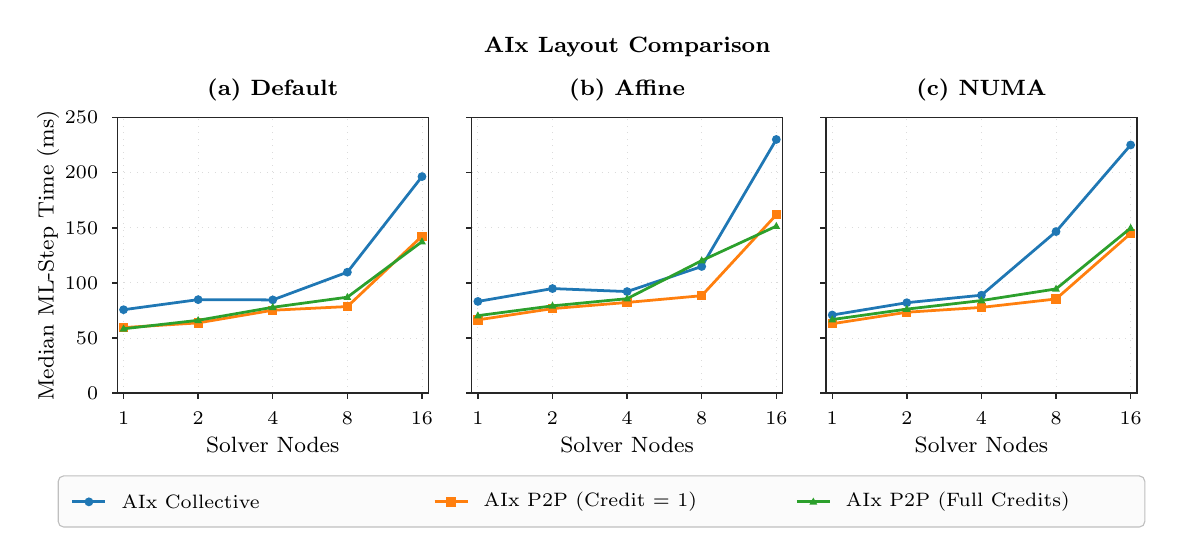
\begin{tikzpicture}[font=\fontsize{8}{10}\selectfont,
axis/.style={black!85,line width=0.5pt},
grid/.style={black!14,line width=0.35pt,dotted},
tick/.style={font=\fontsize{7}{8.5}\selectfont},
title/.style={font=\fontsize{8}{10}\selectfont\bfseries}]
\definecolor{caix_coll}{HTML}{1F77B4}
\definecolor{caix_p2p}{HTML}{FF7F0E}
\definecolor{caix_p2p_fc}{HTML}{2CA02C}
\definecolor{cphydll_default}{HTML}{008080}
\definecolor{cphydll_readiness}{HTML}{17BECF}
\definecolor{csmartsim_c0}{HTML}{D62728}
\definecolor{csmartsim_c3}{HTML}{9467BD}
\definecolor{csmartsim_per_gpu_db}{HTML}{8C564B}
\node[title] at (6.475,4.400) {AIx Layout Comparison};
\begin{scope}[shift={(0.000,0)}]
\node[title] at (1.975,3.850) {(a) Default};
\draw[grid] (0,0.0000) -- (3.950,0.0000);
\draw[axis] (0,0.0000) -- (-0.07,0.0000);
\node[tick,anchor=east] at (-0.12,0.0000) {0};
\draw[grid] (0,0.7000) -- (3.950,0.7000);
\draw[axis] (0,0.7000) -- (-0.07,0.7000);
\node[tick,anchor=east] at (-0.12,0.7000) {50};
\draw[grid] (0,1.4000) -- (3.950,1.4000);
\draw[axis] (0,1.4000) -- (-0.07,1.4000);
\node[tick,anchor=east] at (-0.12,1.4000) {100};
\draw[grid] (0,2.1000) -- (3.950,2.1000);
\draw[axis] (0,2.1000) -- (-0.07,2.1000);
\node[tick,anchor=east] at (-0.12,2.1000) {150};
\draw[grid] (0,2.8000) -- (3.950,2.8000);
\draw[axis] (0,2.8000) -- (-0.07,2.8000);
\node[tick,anchor=east] at (-0.12,2.8000) {200};
\draw[grid] (0,3.5000) -- (3.950,3.5000);
\draw[axis] (0,3.5000) -- (-0.07,3.5000);
\node[tick,anchor=east] at (-0.12,3.5000) {250};
\draw[grid] (0.0800,0) -- (0.0800,3.5);
\draw[axis] (0.0800,0) -- (0.0800,-0.07);
\node[tick,anchor=north] at (0.0800,-0.12) {1};
\draw[grid] (1.0275,0) -- (1.0275,3.5);
\draw[axis] (1.0275,0) -- (1.0275,-0.07);
\node[tick,anchor=north] at (1.0275,-0.12) {2};
\draw[grid] (1.9750,0) -- (1.9750,3.5);
\draw[axis] (1.9750,0) -- (1.9750,-0.07);
\node[tick,anchor=north] at (1.9750,-0.12) {4};
\draw[grid] (2.9225,0) -- (2.9225,3.5);
\draw[axis] (2.9225,0) -- (2.9225,-0.07);
\node[tick,anchor=north] at (2.9225,-0.12) {8};
\draw[grid] (3.8700,0) -- (3.8700,3.5);
\draw[axis] (3.8700,0) -- (3.8700,-0.07);
\node[tick,anchor=north] at (3.8700,-0.12) {16};
\node at (1.975,-0.65) {Solver Nodes};
\node[rotate=90] at (-0.88,1.750) {Median ML-Step Time (ms)};
\begin{scope}
\clip (0,0) rectangle (3.95,3.5);
% aix_coll_default: 75.72750, 84.86250, 84.62150, 109.77150, 196.49100 ms
\draw[caix_coll,line width=1pt,solid] (0.0800,1.0602) -- (1.0275,1.1881) -- (1.9750,1.1847) -- (2.9225,1.5368) -- (3.8700,2.7509);
\fill[caix_coll] (0.0800,1.0602) circle (1.6pt);
\fill[caix_coll] (1.0275,1.1881) circle (1.6pt);
\fill[caix_coll] (1.9750,1.1847) circle (1.6pt);
\fill[caix_coll] (2.9225,1.5368) circle (1.6pt);
\fill[caix_coll] (3.8700,2.7509) circle (1.6pt);
% aix_p2p_default: 59.50500, 63.78200, 75.25750, 78.57900, 142.44900 ms
\draw[caix_p2p,line width=1pt,solid] (0.0800,0.8331) -- (1.0275,0.8929) -- (1.9750,1.0536) -- (2.9225,1.1001) -- (3.8700,1.9943);
\draw[caix_p2p,fill=caix_p2p,line width=0.8pt] (0.0350,0.7881) rectangle (0.1250,0.8781);
\draw[caix_p2p,fill=caix_p2p,line width=0.8pt] (0.9825,0.8479) rectangle (1.0725,0.9379);
\draw[caix_p2p,fill=caix_p2p,line width=0.8pt] (1.9300,1.0086) rectangle (2.0200,1.0986);
\draw[caix_p2p,fill=caix_p2p,line width=0.8pt] (2.8775,1.0551) rectangle (2.9675,1.1451);
\draw[caix_p2p,fill=caix_p2p,line width=0.8pt] (3.8250,1.9493) rectangle (3.9150,2.0393);
% aix_p2p_fc_default: 58.41950, 66.12700, 77.93550, 87.08700, 137.45400 ms
\draw[caix_p2p_fc,line width=1pt,solid] (0.0800,0.8179) -- (1.0275,0.9258) -- (1.9750,1.0911) -- (2.9225,1.2192) -- (3.8700,1.9244);
\fill[caix_p2p_fc] (0.0800,0.8729) -- (0.0300,0.7829) -- (0.1300,0.7829) -- cycle;
\fill[caix_p2p_fc] (1.0275,0.9808) -- (0.9775,0.8908) -- (1.0775,0.8908) -- cycle;
\fill[caix_p2p_fc] (1.9750,1.1461) -- (1.9250,1.0561) -- (2.0250,1.0561) -- cycle;
\fill[caix_p2p_fc] (2.9225,1.2742) -- (2.8725,1.1842) -- (2.9725,1.1842) -- cycle;
\fill[caix_p2p_fc] (3.8700,1.9794) -- (3.8200,1.8894) -- (3.9200,1.8894) -- cycle;
\end{scope}
\draw[axis] (0,0) rectangle (3.95,3.5);
\end{scope}
\begin{scope}[shift={(4.500,0)}]
\node[title] at (1.975,3.850) {(b) Affine};
\draw[grid] (0,0.0000) -- (3.950,0.0000);
\draw[axis] (0,0.0000) -- (-0.07,0.0000);
\draw[grid] (0,0.7000) -- (3.950,0.7000);
\draw[axis] (0,0.7000) -- (-0.07,0.7000);
\draw[grid] (0,1.4000) -- (3.950,1.4000);
\draw[axis] (0,1.4000) -- (-0.07,1.4000);
\draw[grid] (0,2.1000) -- (3.950,2.1000);
\draw[axis] (0,2.1000) -- (-0.07,2.1000);
\draw[grid] (0,2.8000) -- (3.950,2.8000);
\draw[axis] (0,2.8000) -- (-0.07,2.8000);
\draw[grid] (0,3.5000) -- (3.950,3.5000);
\draw[axis] (0,3.5000) -- (-0.07,3.5000);
\draw[grid] (0.0800,0) -- (0.0800,3.5);
\draw[axis] (0.0800,0) -- (0.0800,-0.07);
\node[tick,anchor=north] at (0.0800,-0.12) {1};
\draw[grid] (1.0275,0) -- (1.0275,3.5);
\draw[axis] (1.0275,0) -- (1.0275,-0.07);
\node[tick,anchor=north] at (1.0275,-0.12) {2};
\draw[grid] (1.9750,0) -- (1.9750,3.5);
\draw[axis] (1.9750,0) -- (1.9750,-0.07);
\node[tick,anchor=north] at (1.9750,-0.12) {4};
\draw[grid] (2.9225,0) -- (2.9225,3.5);
\draw[axis] (2.9225,0) -- (2.9225,-0.07);
\node[tick,anchor=north] at (2.9225,-0.12) {8};
\draw[grid] (3.8700,0) -- (3.8700,3.5);
\draw[axis] (3.8700,0) -- (3.8700,-0.07);
\node[tick,anchor=north] at (3.8700,-0.12) {16};
\node at (1.975,-0.65) {Solver Nodes};
\begin{scope}
\clip (0,0) rectangle (3.95,3.5);
% aix_coll_affine: 83.24450, 94.90800, 92.18550, 114.95150, 230.16050 ms
\draw[caix_coll,line width=1pt,solid] (0.0800,1.1654) -- (1.0275,1.3287) -- (1.9750,1.2906) -- (2.9225,1.6093) -- (3.8700,3.2222);
\fill[caix_coll] (0.0800,1.1654) circle (1.6pt);
\fill[caix_coll] (1.0275,1.3287) circle (1.6pt);
\fill[caix_coll] (1.9750,1.2906) circle (1.6pt);
\fill[caix_coll] (2.9225,1.6093) circle (1.6pt);
\fill[caix_coll] (3.8700,3.2222) circle (1.6pt);
% aix_p2p_affine: 66.52550, 76.72650, 82.31800, 88.42700, 161.82400 ms
\draw[caix_p2p,line width=1pt,solid] (0.0800,0.9314) -- (1.0275,1.0742) -- (1.9750,1.1525) -- (2.9225,1.2380) -- (3.8700,2.2655);
\draw[caix_p2p,fill=caix_p2p,line width=0.8pt] (0.0350,0.8864) rectangle (0.1250,0.9764);
\draw[caix_p2p,fill=caix_p2p,line width=0.8pt] (0.9825,1.0292) rectangle (1.0725,1.1192);
\draw[caix_p2p,fill=caix_p2p,line width=0.8pt] (1.9300,1.1075) rectangle (2.0200,1.1975);
\draw[caix_p2p,fill=caix_p2p,line width=0.8pt] (2.8775,1.1930) rectangle (2.9675,1.2830);
\draw[caix_p2p,fill=caix_p2p,line width=0.8pt] (3.8250,2.2205) rectangle (3.9150,2.3105);
% aix_p2p_fc_affine: 70.32500, 79.23350, 85.73000, 120.26050, 151.49900 ms
\draw[caix_p2p_fc,line width=1pt,solid] (0.0800,0.9846) -- (1.0275,1.1093) -- (1.9750,1.2002) -- (2.9225,1.6836) -- (3.8700,2.1210);
\fill[caix_p2p_fc] (0.0800,1.0395) -- (0.0300,0.9496) -- (0.1300,0.9496) -- cycle;
\fill[caix_p2p_fc] (1.0275,1.1643) -- (0.9775,1.0743) -- (1.0775,1.0743) -- cycle;
\fill[caix_p2p_fc] (1.9750,1.2552) -- (1.9250,1.1652) -- (2.0250,1.1652) -- cycle;
\fill[caix_p2p_fc] (2.9225,1.7386) -- (2.8725,1.6486) -- (2.9725,1.6486) -- cycle;
\fill[caix_p2p_fc] (3.8700,2.1760) -- (3.8200,2.0860) -- (3.9200,2.0860) -- cycle;
\end{scope}
\draw[axis] (0,0) rectangle (3.95,3.5);
\end{scope}
\begin{scope}[shift={(9.000,0)}]
\node[title] at (1.975,3.850) {(c) NUMA};
\draw[grid] (0,0.0000) -- (3.950,0.0000);
\draw[axis] (0,0.0000) -- (-0.07,0.0000);
\draw[grid] (0,0.7000) -- (3.950,0.7000);
\draw[axis] (0,0.7000) -- (-0.07,0.7000);
\draw[grid] (0,1.4000) -- (3.950,1.4000);
\draw[axis] (0,1.4000) -- (-0.07,1.4000);
\draw[grid] (0,2.1000) -- (3.950,2.1000);
\draw[axis] (0,2.1000) -- (-0.07,2.1000);
\draw[grid] (0,2.8000) -- (3.950,2.8000);
\draw[axis] (0,2.8000) -- (-0.07,2.8000);
\draw[grid] (0,3.5000) -- (3.950,3.5000);
\draw[axis] (0,3.5000) -- (-0.07,3.5000);
\draw[grid] (0.0800,0) -- (0.0800,3.5);
\draw[axis] (0.0800,0) -- (0.0800,-0.07);
\node[tick,anchor=north] at (0.0800,-0.12) {1};
\draw[grid] (1.0275,0) -- (1.0275,3.5);
\draw[axis] (1.0275,0) -- (1.0275,-0.07);
\node[tick,anchor=north] at (1.0275,-0.12) {2};
\draw[grid] (1.9750,0) -- (1.9750,3.5);
\draw[axis] (1.9750,0) -- (1.9750,-0.07);
\node[tick,anchor=north] at (1.9750,-0.12) {4};
\draw[grid] (2.9225,0) -- (2.9225,3.5);
\draw[axis] (2.9225,0) -- (2.9225,-0.07);
\node[tick,anchor=north] at (2.9225,-0.12) {8};
\draw[grid] (3.8700,0) -- (3.8700,3.5);
\draw[axis] (3.8700,0) -- (3.8700,-0.07);
\node[tick,anchor=north] at (3.8700,-0.12) {16};
\node at (1.975,-0.65) {Solver Nodes};
\begin{scope}
\clip (0,0) rectangle (3.95,3.5);
% aix_coll_numa: 70.91350, 82.08450, 88.89350, 146.59200, 225.17500 ms
\draw[caix_coll,line width=1pt,solid] (0.0800,0.9928) -- (1.0275,1.1492) -- (1.9750,1.2445) -- (2.9225,2.0523) -- (3.8700,3.1524);
\fill[caix_coll] (0.0800,0.9928) circle (1.6pt);
\fill[caix_coll] (1.0275,1.1492) circle (1.6pt);
\fill[caix_coll] (1.9750,1.2445) circle (1.6pt);
\fill[caix_coll] (2.9225,2.0523) circle (1.6pt);
\fill[caix_coll] (3.8700,3.1524) circle (1.6pt);
% aix_p2p_numa: 63.01750, 73.44750, 77.81050, 85.47300, 144.89200 ms
\draw[caix_p2p,line width=1pt,solid] (0.0800,0.8822) -- (1.0275,1.0283) -- (1.9750,1.0893) -- (2.9225,1.1966) -- (3.8700,2.0285);
\draw[caix_p2p,fill=caix_p2p,line width=0.8pt] (0.0350,0.8372) rectangle (0.1250,0.9272);
\draw[caix_p2p,fill=caix_p2p,line width=0.8pt] (0.9825,0.9833) rectangle (1.0725,1.0733);
\draw[caix_p2p,fill=caix_p2p,line width=0.8pt] (1.9300,1.0443) rectangle (2.0200,1.1343);
\draw[caix_p2p,fill=caix_p2p,line width=0.8pt] (2.8775,1.1516) rectangle (2.9675,1.2416);
\draw[caix_p2p,fill=caix_p2p,line width=0.8pt] (3.8250,1.9835) rectangle (3.9150,2.0735);
% aix_p2p_fc_numa: 66.81000, 76.26150, 84.02450, 94.57050, 149.83150 ms
\draw[caix_p2p_fc,line width=1pt,solid] (0.0800,0.9353) -- (1.0275,1.0677) -- (1.9750,1.1763) -- (2.9225,1.3240) -- (3.8700,2.0976);
\fill[caix_p2p_fc] (0.0800,0.9903) -- (0.0300,0.9003) -- (0.1300,0.9003) -- cycle;
\fill[caix_p2p_fc] (1.0275,1.1227) -- (0.9775,1.0327) -- (1.0775,1.0327) -- cycle;
\fill[caix_p2p_fc] (1.9750,1.2313) -- (1.9250,1.1413) -- (2.0250,1.1413) -- cycle;
\fill[caix_p2p_fc] (2.9225,1.3790) -- (2.8725,1.2890) -- (2.9725,1.2890) -- cycle;
\fill[caix_p2p_fc] (3.8700,2.1526) -- (3.8200,2.0626) -- (3.9200,2.0626) -- cycle;
\end{scope}
\draw[axis] (0,0) rectangle (3.95,3.5);
\end{scope}
\draw[black!25,fill=gray!3,rounded corners=2pt] (-0.75,-1.7) rectangle (13.050,-1.05);
\draw[caix_coll,line width=1pt,solid] (-0.570,-1.380) -- (-0.150,-1.380);
\fill[caix_coll] (-0.3600,-1.3800) circle (1.6pt);
\node[anchor=west,font=\fontsize{7}{8.5}\selectfont] at (-0.070,-1.380) {AIx Collective};
\draw[caix_p2p,line width=1pt,solid] (4.030,-1.380) -- (4.450,-1.380);
\draw[caix_p2p,fill=caix_p2p,line width=0.8pt] (4.1950,-1.4250) rectangle (4.2850,-1.3350);
\node[anchor=west,font=\fontsize{7}{8.5}\selectfont] at (4.530,-1.380) {AIx P2P (Credit = 1)};
\draw[caix_p2p_fc,line width=1pt,solid] (8.630,-1.380) -- (9.050,-1.380);
\fill[caix_p2p_fc] (8.8400,-1.3250) -- (8.7900,-1.4150) -- (8.8900,-1.4150) -- cycle;
\node[anchor=west,font=\fontsize{7}{8.5}\selectfont] at (9.130,-1.380) {AIx P2P (Full Credits)};
\end{tikzpicture}
\end{document}
